\chapter{Jet Reconstruction}\label{chapter4}

After the process of the splitting and branching, the quarks and gluons start to hadronize leading to a collimated spray of stable colourless hadrons. Hence in practice
%\Jnote{I don't think ``in practice'' is good choice of words. I would
%  say ``the only directly observed outcome''.}
the only outcome of this process is hadrons \ref{Lhc}. In order to study the quarks and the gluons, it is plausible to think of reversing this process. This process is called jet reconstruction, and the final outcome is called jets (quarks or gluons).     

The jet reconstruction is essential in understanding the link between the observed physics or the long distance physics and the underlying physics (short distance physics) in the parton level.
 %Also, the accurate reconstruction is very important in comparing the theoretical predictions and the data. 

The definition of the jet is central in comparing the data and the theoretical predictions. The definition is provided in the form of the jet algorithm, this means the jet algorithm and its corresponding parameters and recombination scheme.
% The paragraphs below gives a detailed description of the algorithm. 
%In 
%The concrete definition of what is the collimated spray is provided by the \textit{the jet clustering algorithm} \citep{Ellis:2007ib}.    

%The QCD calculations provide a description of a final state in terms of the quark and gluons, however, in practical and due to confinement phenomenon those quarks and gluons can not be observed, the detectors can only observe those stable colourless hadrons. 



%This mapping between the stable hadrons(observed physics) and the partons(unobserved) from the hard scattering is done by the means of the jet algorithms. 

%Jet algorithms basically rely on merging. This means that they merge objects that are near to each other.  As for the accuracy of the algorithm, we assume that the kinematics of the clustered jet provide a useful measure of the kinematics of the underlying short distance physics. In particular, we assume the basic mismatch between the long observed hadrons and short distance unobserved partons which does present any numerical limitations \citep{Ellis:2007ib}. 

    
%The definition of the jet is central in comparing the data and the theoretical predictions, the definition is provided in the form of the jet algorithm, this means the jet algorithm and its corresponding parameters and recombination scheme, we will talk more about this in the following. In this part of the essay we will talk a bout the general idea of the jet algorithms and some of their properties and we will focus on one of them, the $anti-k_{t}$ and it is implementation in python.  

\section{Jet Algorithms}

There are two broad classes of jet algorithms, the Cone algorithms and the Sequential algorithms. Both algorithms work on defining the jets by the idea of nearness.

It is important to recognize that jet algorithms involve two distinct steps. The first step is to identify the members of the jet, i.e., the partons that make-up the final stable jets. The second step is to construct the kinematic properties that will characterize the jet \citep{Berger:2002jt}. For merging and combining the objects, we use the 4 -vector recombination scheme, whereby to combine two particles we add their four momenta \citep{Blazey:2000qt}. 

Here, we will focus on the second class:
%\Jnote{Put colon here.}
the sequential algorithms.  

%\section{The Cone Algorithms}
%The cone algorithms associate hadrons into jets by identifying those that are nearby in angle, $i.e$, they follow the geometrical intuition in defining the jets, where the jet is composed of hadrons and partons whose momenta lie within a cone defined by  a circle in $\eta-\phi$ plane. Where $\eta$ is the pseudo-rapidity and can be calculated by $\ln(\cot \frac{\phi}{2})$, and $\phi$ is the azimuthal angle \citep{Berger:2002jt}. 
%
%For the first step in the algorithm, \textit{i.e}, identifying the members of the jet, it is a simple sum over the all (short and long distances) within a cone centred at $\eta-\phi$ plane. Here, one introduces the concept of \textit{stable} cones as a circle of fixed radius \textit{R} in the plane $\eta-\phi$ such that the sum of all four momenta within the cone points to the same direction as the centre of the circle. The cone algorithms attempts to identify the stable cones. Thus, at least in principle one can think in terms of placing trial cones randomly in the plane $\eta-\phi$  and allowing them to follow until a stable cone or a jet is found \citep{Ellis:2007ib}.
%
%Cone algorithms differ in the way they deal with the fact that the stable cones may overlap. There are two famous cone algorithms. They are, the midpoint cone algorithm and SISCone (seedless infra-red safe cone) \citep{Ellis:2007ib}.  
\section{Sequential Algorithms}

These algorithms work by defining a distance between pairs of objects, performing a successive recombination of the pair of closest objects, and stopping when all objects are far apart.
%\Jnote{s/further apart/far apart}

One starts by first defining these distances, $d_{ij}$ \eqref{dij} and $d_{iB}$ \eqref{dib}, where $d_{ij}$ is the distance between objects (pseudo-jets)\footnote{Pseudo-jet since it is neither a full jet, nor yet a full particle. It can be a single particle or a composition of particles.}
%\Jnote{In footnote:s/full particle/full jet}
$i$ and $j$, and $d_{iB}$ is the distance between the pseudo-jet $i$ and the beam B. The clustering proceeds by identifying the smallest of the distances and if it is $d_{ij}$ combine the pseudo-jets $i$ and $j$. Otherwise, if it is $d_{iB}$ calling $i$ a jet and removing it from the list of objects. The distances are recalculated and the procedure repeated until no objects are left \citep{Cacciari:2008gp}. 

The difference between the sequential algorithms lies in the definition of the distances measures:
\begin{equation}
d_{ij} = \min(k_{ti}^{2p}, k_{tj}^{2p}) \frac{\Delta_{ij}}{R^{2}},
\label{dij}\end{equation}         
\begin{equation}
d_{iB} = k_{ti}^{2p} ,
\label{dib}\end{equation}
%\Jnote{Use \textbackslash min in math mode to get nicer font.}
Where $\Delta_{ij}^{2} = (y_{i} - y_{j})^2 + (\phi_{i} - \phi_{j})^2$ and $k_{ti}$, $\eta_{i}$ and $\phi_{i}$ are the transverse momentum, rapidity and  the azimuth of the particle $i$ \citep{Cacciari:2008gp}. The exact formula for the transverse momentum depends on the beam axis, which is $z$ hence, $k_{t} = \sqrt{p_x^2 + p_y^2}$. The rapidity describes the angle relative to the beam axis.
%It is defined as $- \ln \left[\tan\left(\frac{\theta}{2}\right)\right]$ where $\theta$ is the polar angle  \citep{Salam:2009jx}. 
The rapidity is defined as $\frac{1}{2} \ln \frac{E_i + p_{zi}}{E_i - p_{zi}}$, where  $E_i$ and $p_{zi}$ are the energy and component of the momentum along the beam axis of the particle $i$ \citep{Cacciari:2011ma}. The parameter $R$ describes the jet radius. 
%, it is a parameter of the algorithm that determines its angular reach \citep{Cacciari:2011ma}.
%The parameter $p$ govern the relative of the energy versus geometrical ($\Delta_{ij}$ scales \citep{Cacciari:2008gp}. 

The inclusive $k_t$ algorithm is defined with choice of $p = 1$, the case where $p = 0$  corresponds to the inclusive Cambridge/Aachen algorithm, where $p = -1$ refers to anti-$k_t$ jet clustering algorithm \citep{Cacciari:2008gp}.
%\Jnote{Rephrase: ``If $p$ is chosen to be one, the resulting algorithm
%  is called inclusive $k_t$ algorithm'' etc.}

%\Jnote{Consider adding some sentences on that would help to intuitively understand
%  the formulas. For example:
%  When are two jets close for $p=-1$? When are they close for $p=1$?
%  What happens to number of jets as $R$ varies?}

%The behaviours of different jet algorithms are illustrated in figure \ref{fig:jets} where a parton level event has been taken together with random soft (radiated) particles and then clustered with 4 different jet algorithms. The figure shows the region which within the random soft particles are clustered. For the $k_t$ and Cambridge/Aachen algorithms, that region depends somewhat on the specific set of soft particles and the irregular borders of the jet are consequence of the randomness of the soft particles.
% For SISCone it can be seen that single-particle jets are regular (though with a radius $R/2$), while composite jets have varied shapes. 
% With the anti-$k_t$ algorithms, the hard jets are circular and the softer jets have more complex shapes. The pair of jets near $\phi = 5$ and $y = - 2$ provides an example in this respect. The former is much softer than the later. The circular hard jets clips a lens shaped region out of the soft one, creating the crescent shape \citep{Cacciari:2008gp}.                
%%\begin{figure}[H]
%%
%\centering
%
%\begin{subfigure}[b]{0.3 \textwidth}
%
%  \centering
%
%  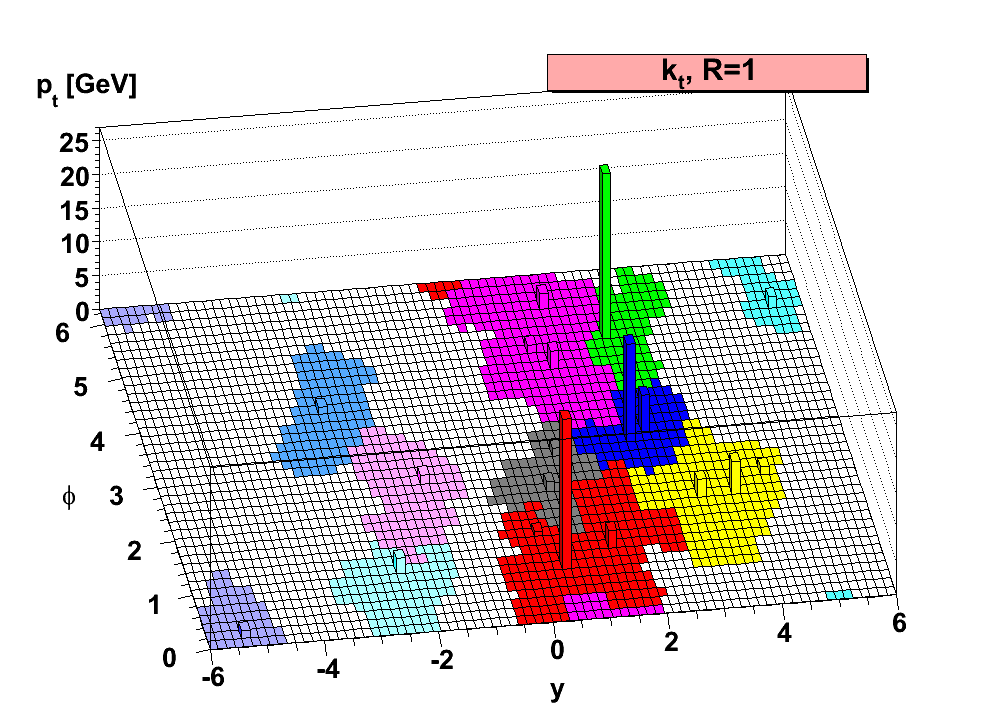
\includegraphics[width = \textwidth]{images/ff1.png}
%
%  %\caption{Neurons, Erdos,barabasi and watts}
%
%  \label{fig:a1}
%
%\end{subfigure}
%
%\begin{subfigure}[b]{0.3 \textwidth}
%
%  \centering
%
%  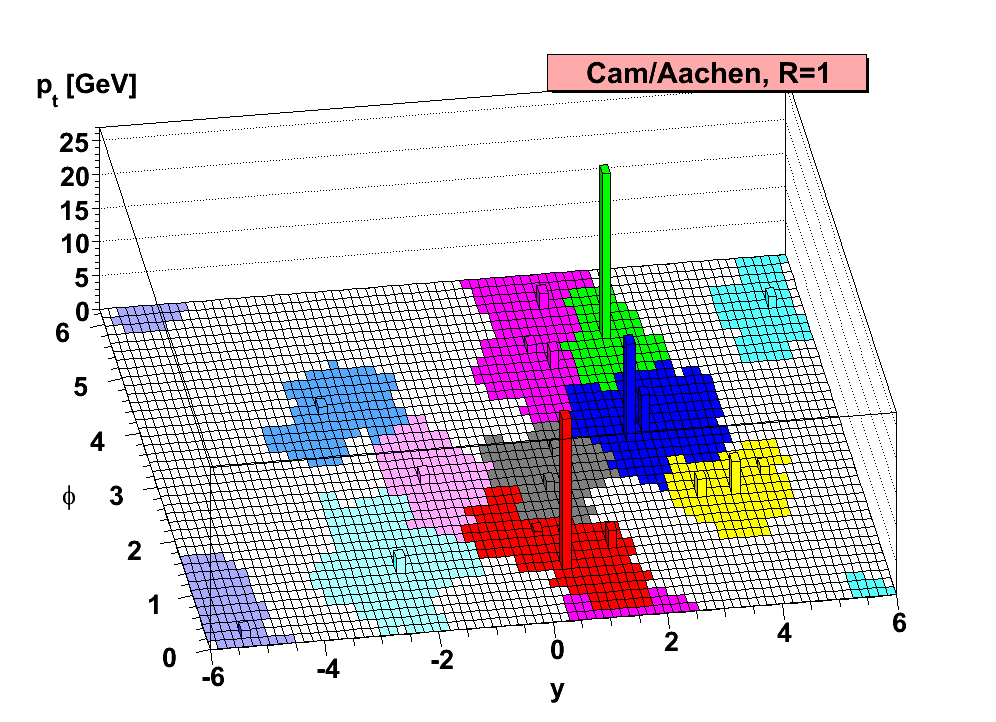
\includegraphics[width = \textwidth]{images/ff.png}
%
%  %\caption{scotch broom, Erdos,barabasi and watts}
%
% \label{fig:b1}
%
%\end{subfigure}
%
%\begin{subfigure}[b]{0.3 \textwidth}
%
% \centering
%
%  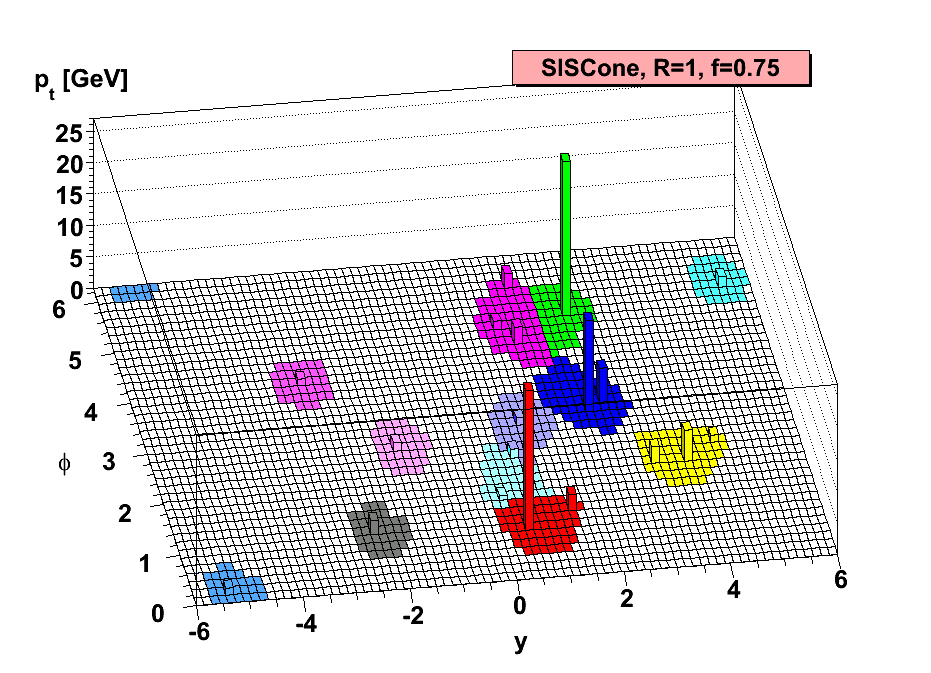
\includegraphics[width = \textwidth]{images/ff2.png}
%
% %\caption{citation, Erdos,barabasi and watts}
%
%  \label{fig:c1}
%
%\end{subfigure}
%
%\begin{subfigure}[b]{0.3 \textwidth}
%
%  \centering
%
%  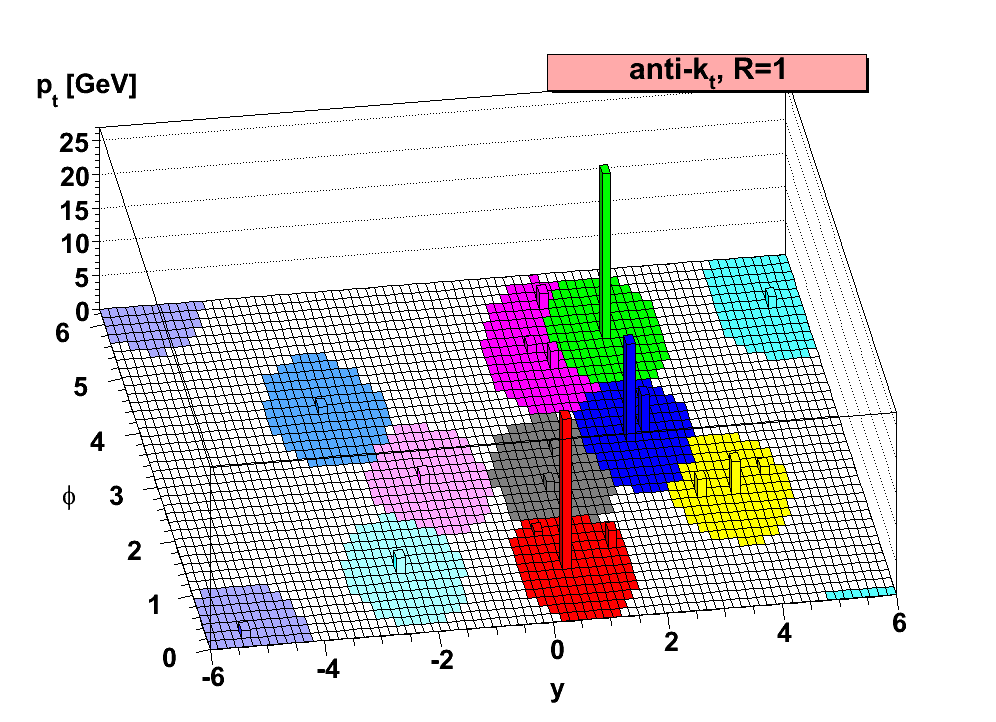
\includegraphics[width = \textwidth]{images/ff3.png}
%
%  %\caption{Malaria, Erdos,barabasi and watts}
%
%  \label{fig:d1}
%
%\end{subfigure}
%

%
%\caption{A sample parton-level event (generated with Herwig), together with many random soft
%, clustered with four different jets algorithms, illustrating the “active” catchment areas of
%the resulting hard jets.}
%
%  \label{fig:jets}
%
%\end{figure}
%
%\begin{figure}[h!]
%    \centering
%    \begin{subfigure}[h!]{0.495\textwidth}
%        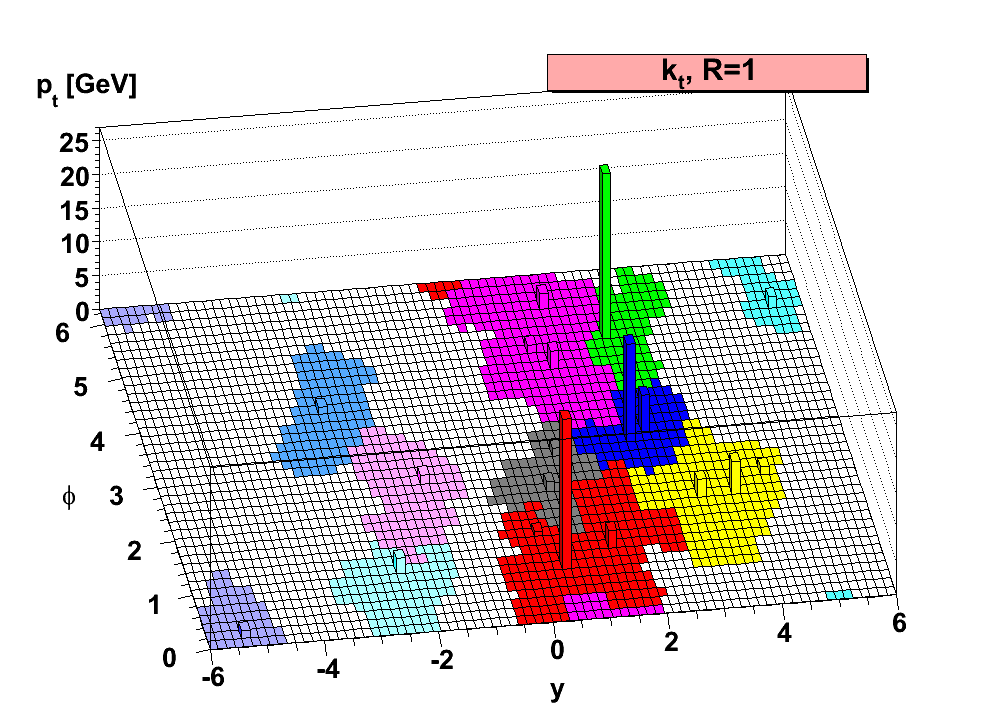
\includegraphics[width=\textwidth]{images/ff1.png}
%        \label{fig:gull}
%    \end{subfigure}
%    \begin{subfigure}[h!]{0.495\textwidth}
%        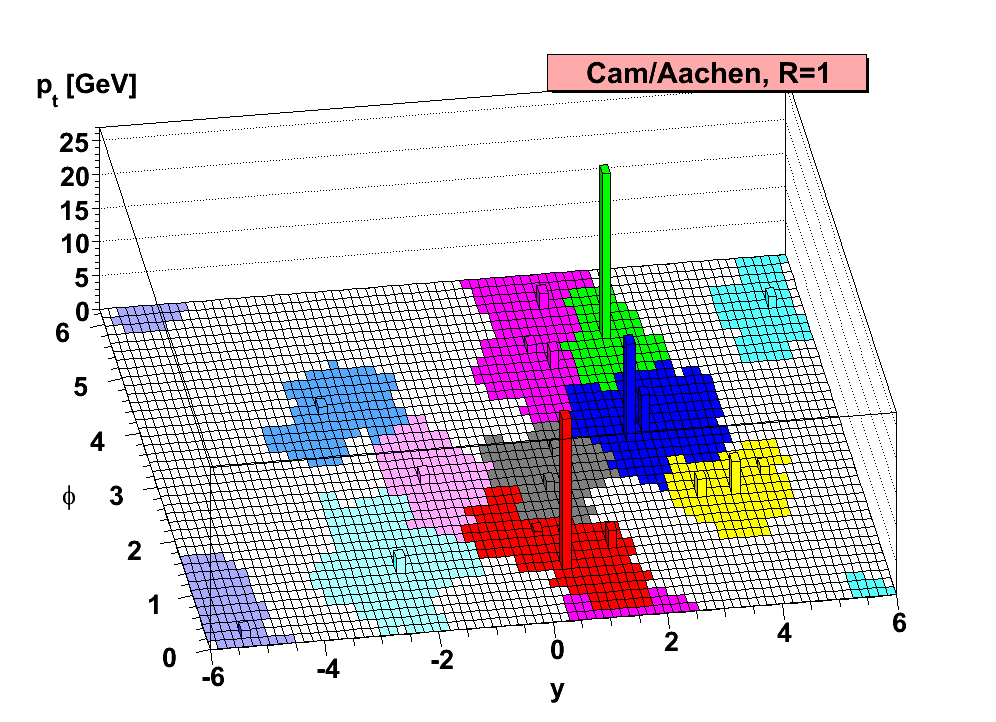
\includegraphics[width=\textwidth]{images/ff.png}
%        \label{fig:mouse}
%    \end{subfigure}
%    \begin{subfigure}[h!]{0.495\textwidth}
%        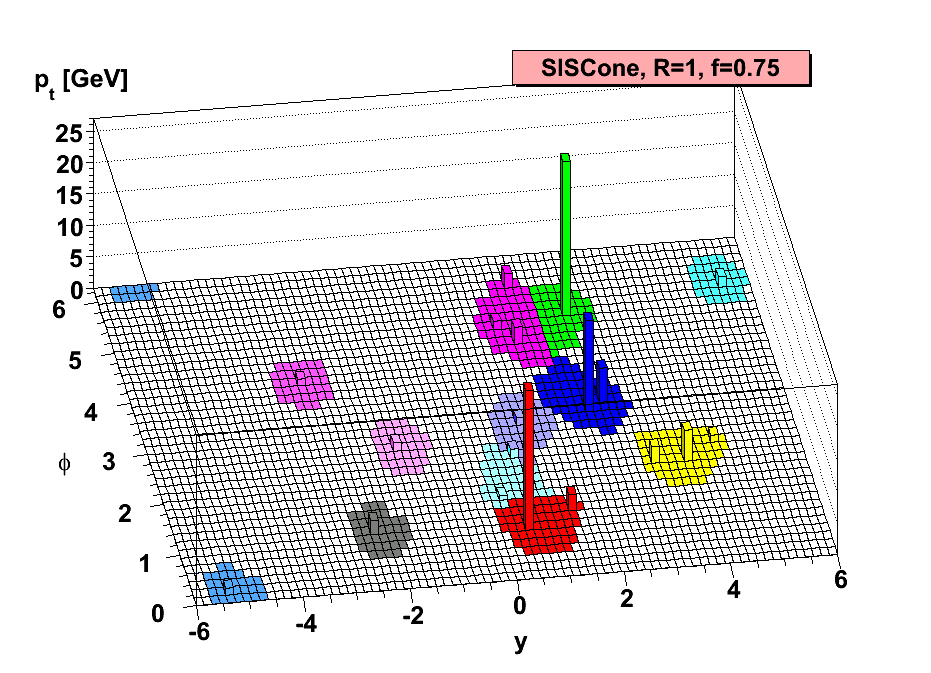
\includegraphics[width=\textwidth]{images/ff2.png}
%        \label{fig:mouse}
%    \end{subfigure}
%        \begin{subfigure}[h!]{0.495\textwidth}
%        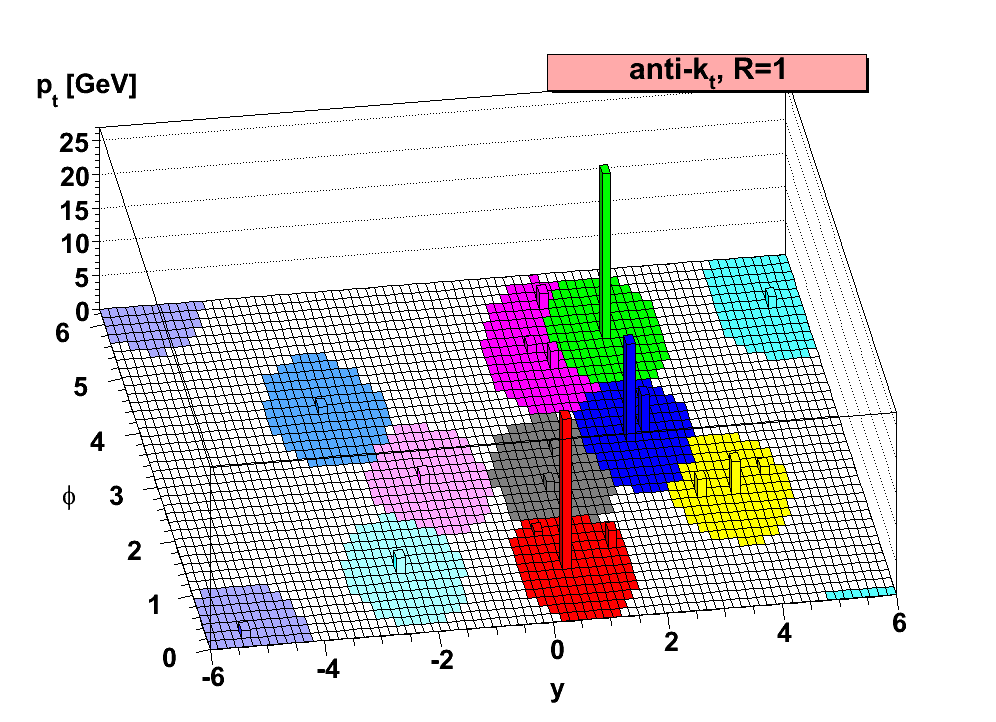
\includegraphics[width=\textwidth]{images/ff3.png}
%        \label{fig:mouse}
%    \end{subfigure}
%
%    \caption{A sample parton-level event (generated with Herwig), together with many random soft, clustered with four different jets algorithms, illustrating the “active” catchment areas of
%the resulting hard jets.}\label{fig:jets}
%\end{figure}

%\section{Implementation of Anti-$k_t$}

The implementation of anti-$k_t$ clustering algorithm can be illustrated by the following pseudocode
%\Jnote{s/algorithm/pseudocode}
\begin{algorithmic}
\State Calculate all the $d_{ij}$ and $d_{iB}$
\State Find the minimum of $d_{ij}$ and $d_{iB}$ 
\If {minimum distance is $d_{ij}$}
	\State Recombine $i$ and $j$ in a single object 
	\State Go to step one
\Else \State the minimum is $d_{iB}$
	\State Declare $i$ as a jet and remove from the list
	\State Start from the beginning	
\EndIf
\State Repeat until no objects left 
\end{algorithmic}
%\Jnote{Better use a loop. Don't say ``return step one''. You can
%  say ``goto step one''. Better yet write a loop such that it's not
%  necessary.}
%The algorithm for this work was implemented in Python. The main step in the algorithm  decides the nature of the object, $i.e$, finding the minimum in the list of the distances. We used the Python function \verb+heap queue+ which is an implementation of the priority queue algorithm. This function gives the smallest element in a list, maintaining the list invariant. 

%For the code and the documentation see \verb+anti_kT_algorithm.py+.